%╔════════════════════════════╗
%║	  Szablon dostosował	  ║
%║	mgr inż. Dawid Kotlarski  ║
%║		  06.10.2024		  ║
%╚════════════════════════════╝
\documentclass[12pt,twoside,a4paper,openany]{article}

    % ------------------------------------------------------------------------
% PAKIETY
% ------------------------------------------------------------------------

%różne pakiety matematyczne, warto przejrzeć dokumentację, muszą być powyżej ustawień językowych.
\usepackage{mathrsfs}   %Różne symbole matematyczne opisane w katalogu ~\doc\latex\comprehensive. Zamienia \mathcal{L} ze zwykłego L na L-transformatę.
\usepackage{eucal}      %Różne symbole matematyczne.
\usepackage{amssymb}    %Różne symbole matematyczne.
\usepackage{amsmath}    %Dodatkowe funkcje matematyczne, np. polecenie \dfac{}{} skladajace ulamek w trybie wystawionym (porównaj $\dfrac{1}{2}$, a $\frac{1}{2}$).

%język polski i klawiatura
\usepackage[polish]{babel}
%\usepackage{qtimes} % czcionka Times new Roman
\usepackage[OT4]{polski}
%\usepackage[cp1250]{inputenc}                       %Strona kodowa polskich znaków.

%obsługa pdf'a
\usepackage[pdftex,usenames,dvipsnames]{color}      %Obsługa kolorów. Opcje usenames i dvipsnames wprowadzają dodatkowe nazwy kolorow.
\usepackage[pdftex,pagebackref=false,draft=false,pdfpagelabels=false,colorlinks=true,urlcolor=blue,linkcolor=black,citecolor=green,pdfstartview=FitH,pdfstartpage=1,pdfpagemode=UseOutlines,bookmarks=true,bookmarksopen=true,bookmarksopenlevel=2,bookmarksnumbered=true,pdfauthor={Dawid Kotlarski},pdftitle={Dokumentacja Projektowa},pdfsubject={},pdfkeywords={transient recovery voltage trv},unicode=true]{hyperref}   %Opcja pagebackref=true dotyczy bibliografii: pokazuje w spisie literatury numery stron, na których odwołano się do danej pozycji.

%bibliografia
%\usepackage[numbers,sort&compress]{natbib}  %Porządkuje zawartość odnośników do literatury, np. [2-4,6]. Musi być pod pdf'em, a styl bibliogfafii musi mieć nazwę z dodatkiem 'nat', np. \bibliographystyle{unsrtnat} (w kolejności cytowania).
\usepackage[
backend=biber,
style=numeric,
sorting=none
]{biblatex}
\addbibresource{bibliografia.bib}
\usepackage{hypernat}                       %Potrzebna pakietowi natbib do wspolpracy z pakietem hyperref (wazna kolejnosc: 1. hyperref, 2. natbib, 3. hypernat).

%grafika i geometria strony
\usepackage{extsizes}           %Dostepne inne rozmiary czcionek, np. 14 w poleceniu: \documentclass[14pt]{article}.
\usepackage[final]{graphicx}
\usepackage[a4paper,left=3.5cm,right=2.5cm,top=2.5cm,bottom=2.5cm]{geometry}

%strona tytułowa
\usepackage{strona_tytulowa}

%inne
\usepackage[hide]{todo}                     %Wprowadza polecenie \todo{treść}. Opcje pakietu: hide/show. Polecenie \todos ma byc na koncu dokumentu, wszystkie \todo{} po \todos sa ignorowane.
\usepackage[basic,physics]{circ}            %Wprowadza środowisko circuit do rysowania obwodów elektrycznych. Musi byc poniżej pakietow językowych.
\usepackage[sf,bf,outermarks]{titlesec}     %Troszczy się o wygląd tytułów rozdziałów (section, subsection, ...). sf oznacza czcionkę sans serif (typu arial), bf -- bold. U mnie: oddzielna linia dla naglowku paragraph. Patrz tez: tocloft -- lepiej robi format spisu tresci.
\usepackage{tocloft}                        %Troszczy się o format spisu trsci.
\usepackage{expdlist}    %Zmienia definicję środowiska description, daje większe możliwości wpływu na wygląd listy.
\usepackage{flafter}     %Wprowadza parametr [tb] do polecenia \suppressfloats[t] (polecenie to powoduje nie umieszczanie rysunkow, tabel itp. na stronach, na ktorych jest to polecenie (np. moze byc to stroma z tytulem rozdzialu, ktory chcemy zeby byl u samej gory, a nie np. pod rysunkiem)).
\usepackage{array}       %Ładniej drukuje tabelki (np. daje wiecej miejsca w komorkach -- nie są tak ścieśnione, jak bez tego pakietu).
\usepackage{listings}    %Listingi programow.
\usepackage[format=hang,labelsep=period,labelfont={bf,small},textfont=small]{caption}   %Formatuje podpisy pod rysunkami i tabelami. Parametr 'hang' powoduje wcięcie kolejnych linii podpisu na szerokosc nazwy podpisu, np. 'Rysunek 1.'.
\usepackage{appendix}    %Troszczy się o załączniki.
\usepackage{floatflt}    %Troszczy się o oblewanie rysunkow tekstem.
\usepackage{here}        %Wprowadza dodtkowy parametr umiejscowienia rysunków, tabel, itp.: H (duże). Umiejscawia obiekty ruchome dokladnie tam gdzie są w kodzie źródłowym dokumentu.
\usepackage{makeidx}     %Troszczy się o indeks (skorowidz).

%nieużywane, ale potencjalnie przydatne
\usepackage{sectsty}           %Formatuje nagłówki, np. żeby były kolorowe -- polecenie: \allsectionsfont{\color{Blue}}.
%\usepackage{version}           %Wersje dokumentu.

%============
\usepackage{longtable}			%tabelka
%============

%============
% Ustawienia listingów do kodu
%============

\usepackage{listings}
\usepackage{xcolor}

\definecolor{codegreen}{rgb}{0,0.6,0}
\definecolor{codegray}{rgb}{0.5,0.5,0.5}
\definecolor{codepurple}{rgb}{0.58,0,0.82}
\definecolor{backcolour}{rgb}{0.95,0.95,0.92}

% Definicja stylu "mystyle"
\lstdefinestyle{mystyle}{
	backgroundcolor=\color{backcolour},   
	commentstyle=\color{codegreen},
	keywordstyle=\color{blue},	%magenta
	numberstyle=\tiny\color{codegray},
	stringstyle=\color{codepurple},
	basicstyle=\ttfamily\footnotesize,
	breakatwhitespace=false,         
	breaklines=true,                 
	captionpos=b,                    
	keepspaces=true,                 
	numbers=left,                    
	numbersep=5pt,                  
	showspaces=false,                
	showstringspaces=false,
	showtabs=false,                  
	tabsize=2
}

\lstset{style=mystyle} % Deklaracja aktywnego stylu
%===========

%PAGINA GÓRNA I DOLNA
\usepackage{fancyhdr}          %Dodaje naglowki jakie się chce.
\pagestyle{fancy}
\fancyhf{}
% numery stron w paginie dolnej na srodku
\fancyfoot[C]{\scriptsize DOKUMENTACJA PROJEKTU - ZAAWANSOWANE PROGRAMOWANIE \\ 
\normalsize\sffamily  \thepage}


%\fancyhead[L]{\small\sffamily \nouppercase{\leftmark}}
\fancyhead[C]{\footnotesize \textit{AKADEMIA NAUK STOSOWANYCH W NOWYM SĄCZU}\\}

\renewcommand{\headrulewidth}{0.4pt}
\renewcommand{\footrulewidth}{0.4pt}

    % ------------------------------------------------------------------------
% USTAWIENIA
% ------------------------------------------------------------------------

% ------------------------------------------------------------------------
%   Kropki po numerach sekcji, podsekcji, itd.
%   Np. 1.2. Tytuł podrozdziału
% ------------------------------------------------------------------------
\makeatletter
    \def\numberline#1{\hb@xt@\@tempdima{#1.\hfil}}                      %kropki w spisie treści
    \renewcommand*\@seccntformat[1]{\csname the#1\endcsname.\enspace}   %kropki w treści dokumentu
\makeatother

% ------------------------------------------------------------------------
%   Numeracja równań, rysunków i tabel
%   Np.: (1.2), gdzie:
%   1 - numer sekcji, 2 - numer równania, rysunku, tabeli
%   Uwaga ogólna: o otoczeniu figure ma być najpierw \caption{}, potem \label{}, inaczej odnośnik nie działa!
% ------------------------------------------------------------------------
\makeatletter
    \@addtoreset{equation}{section} %resetuje licznik po rozpoczęciu nowej sekcji
    \renewcommand{\theequation}{{\thesection}.\@arabic\c@equation} %dodaje kropki

    \@addtoreset{figure}{section}
    \renewcommand{\thefigure}{{\thesection}.\@arabic\c@figure}

    \@addtoreset{table}{section}
    \renewcommand{\thetable}{{\thesection}.\@arabic\c@table}
\makeatother

% ------------------------------------------------------------------------
% Tablica
% ------------------------------------------------------------------------
\newenvironment{tabela}[3]
{
    \begin{table}[!htb]
    \centering
    \caption[#1]{#2}
    \vskip 9pt
    #3
}{
    \end{table}
}

% ------------------------------------------------------------------------
% Dostosowanie wyglądu pozycji listy \todos, np. zamiast 'p.' jest 'str.'
% ------------------------------------------------------------------------
\renewcommand{\todoitem}[2]{%
    \item \label{todo:\thetodo}%
    \ifx#1\todomark%
        \else\textbf{#1 }%
    \fi%
    (str.~\pageref{todopage:\thetodo})\ #2}
\renewcommand{\todoname}{Do zrobienia...}
\renewcommand{\todomark}{~uzupełnić}

% ------------------------------------------------------------------------
% Definicje
% ------------------------------------------------------------------------
\def\nonumsection#1{%
    \section*{#1}%
    \addcontentsline{toc}{section}{#1}%
    }
\def\nonumsubsection#1{%
    \subsection*{#1}%
    \addcontentsline{toc}{subsection}{#1}%
    }
\reversemarginpar %umieszcza notki po lewej stronie, czyli tam gdzie jest więcej miejsca
\def\notka#1{%
    \marginpar{\footnotesize{#1}}%
    }
\def\mathcal#1{%
    \mathscr{#1}%
    }
\newcommand{\atp}{ATP/EMTP} % Inaczej: \def\atp{ATP/EMTP}

% ------------------------------------------------------------------------
% Inne
% ------------------------------------------------------------------------
\frenchspacing                      
\hyphenation{ATP/-EMTP}             %dzielenie wyrazu w danym miejscu
\setlength{\parskip}{3pt}           %odstęp pomiędzy akapitami
\linespread{1.3}                    %odstęp pomiędzy liniami (interlinia)
\setcounter{tocdepth}{4}            %uwzględnianie w spisie treści czterech poziomów sekcji
\setcounter{secnumdepth}{4}         %numerowanie do czwartego poziomu sekcji 
\titleformat{\paragraph}[hang]      %wygląd nagłówków
{\normalfont\sffamily\bfseries}{\theparagraph}{1em}{}

% Makro do zdjęć
\newcommand*{\fg}[4][!htb]{
    \begin{figure}[#1]
        \begin{center}
            \includegraphics[width=8cm]{#2}
            \caption{#3}
            \label{#4}
        \end{center}
    \end{figure}
}


    %polecenia zdefiniowane w pakiecie strona_tytulowa.sty
    \title{Drzewo Przeszukiwań Binarnych (BST)}		%...Wpisać nazwę projektu...
    \author{Marcin Dudek}
    \authorI{Mateusz Basiaga}
    \authorII{}		%jeśli są dwie osoby w projekcie to zostawiamy:    \authorII{}
		
	\uczelnia{AKADEMIA NAUK STOSOWANYCH \\W NOWYM SĄCZU}
    \instytut{Wydział Nauk Inżynieryjnych}
    \kierunek{Katedra Informatyki}
    \praca{DOKUMENTACJA PROJEKTOWA}
    \przedmiot{ZAAWANSOWANE PROGRAMOWANIE}
    \prowadzacy{mgr inż. Dawid Kotlarski}
    \rok{2024}


%definicja składni mikrotik
\usepackage{fancyvrb}
\DefineVerbatimEnvironment{MT}{Verbatim}%
{commandchars=\+\[\],fontsize=\small,formatcom=\color{red},frame=lines,baselinestretch=1,} 
\let\mt\verb 
%zakonczenie definicji składni mikrotik

\usepackage{fancyhdr}    %biblioteka do nagłówka i stopki

			
\begin{document}

\renewcommand{\figurename}{Rys.}    %musi byc pod \begin{document}, bo w~tym miejscu pakiet 'babel' narzuca swoje ustawienia
\renewcommand{\tablename}{Tab.}     %j.w.
\thispagestyle{empty}               %na tej stronie: brak numeru
\stronatytulowa                     %strona tytułowa tworzona przez pakiet strona_tytulowa.tex

\pagestyle{fancy}

\newpage

%formatowanie spisu treści i~nagłówków
\renewcommand{\cftbeforesecskip}{8pt}
\renewcommand{\cftsecafterpnum}{\vskip 8pt}
\renewcommand{\cftparskip}{3pt}
\renewcommand{\cfttoctitlefont}{\Large\bfseries\sffamily}
\renewcommand{\cftsecfont}{\bfseries\sffamily}
\renewcommand{\cftsubsecfont}{\sffamily}
\renewcommand{\cftsubsubsecfont}{\sffamily}
\renewcommand{\cftparafont}{\sffamily}
%koniec formatowania spisu treści i nagłówków

\tableofcontents    %spis treści
\thispagestyle{fancy}
\newpage


\newpage


%%%%%%%%%%%%%%%%%%% treść główna dokumentu %%%%%%%%%%%%%%%%%%%%%%%%%

\newpage
\section{Ogólne określenie wymagań}

Celem projektu jest stworzenie aplikacji w języku C++ umożliwiającej obsługę drzewa wyszukiwań binarnych (BST - Binary Search Tree) oraz umożliwiającej jego zarządzanie i wizualizację. Projekt realizowany jest z myślą o zdobyciu praktycznego doświadczenia z systemem kontroli wersji GitHub, przy pracy w grupie dwuosobowej, z zastosowaniem narzędzi do zarządzania kodem i dokumentacją.

\subsection{Zakładany efekt końcowy}

Efektem końcowym pracy jest aplikacja spełniająca wymagania funkcjonalne oraz strukturalne określone w specyfikacji. Działanie programu powinno umożliwić:
\begin{itemize}
  \item Dodawanie, usuwanie oraz przeszukiwanie elementów w drzewie binarnym;
  \item Wyświetlanie struktury drzewa w różnych formach porządkowania (preorder, inorder, postorder);
  \item Zapis i odczyt drzewa do/z pliku binarnego oraz tekstowego, co pozwoli na ponowne załadowanie drzewa bez utraty danych;
  \item Wczytanie danych z pliku tekstowego i ich przekształcenie w strukturę drzewa BST, zarówno do pustego drzewa, jak i z możliwością łączenia z już istniejącą strukturą.
\end{itemize}

\subsection{Cele techniczne}

Projekt został zaplanowany tak, aby spełnić poniższe cele techniczne:
\begin{itemize}
  \item Implementacja klasy \texttt{BinarySearchTree} realizującej główne operacje na drzewie BST: dodawanie, usuwanie, przeszukiwanie, wyświetlanie oraz zapis i odczyt z pliku;
  \item Stworzenie dodatkowej klasy \texttt{App} odpowiedzialnej za zarządzanie drzewem poprzez menu interaktywne, obsługujące wybory użytkownika oraz wywołujące odpowiednie operacje na drzewie;
  \item Rozdzielenie kodu źródłowego na moduły zgodnie z zasadami programowania obiektowego, w tym podział na pliki nagłówkowe i implementacyjne, aby ułatwić dalszy rozwój i testowanie kodu;
  \item Wykorzystanie narzędzi GitHub do wersjonowania kodu, pracy równoległej oraz rozwiązywania konfliktów;
  \item Stworzenie dokumentacji projektu z wykorzystaniem narzędzia \texttt{Doxygen} oraz dokumentacji w \LaTeX, aby opisać implementację, działanie oraz wyniki końcowe projektu.
\end{itemize}

\subsection{Wymagania dotyczące kontroli wersji i pracy zespołowej}

W projekcie przewiduje się równoległą pracę dwuosobową, co wiąże się z określonymi wymaganiami:
\begin{itemize}
  \item Utworzenie repozytorium GitHub, które będzie śledzić postępy prac nad projektem;
  \item Każdy z członków zespołu będzie odpowiedzialny za stworzenie nowej gałęzi w projekcie, wykonanie co najmniej 5 commitów i późniejsze połączenie tych zmian z główną gałęzią (tzw. \texttt{merge});
  \item Projekt wymaga rozwiązania co najmniej 6 konfliktów w kodzie podczas łączenia gałęzi, co pozwala zdobyć doświadczenie w rozwiązywaniu problemów wynikających z pracy równoległej w zespole;
  \item Zastosowanie narzędzi GitHub do przeglądu kodu, rozwiązywania konfliktów oraz dokumentowania zmian przy pomocy opisowych commitów.
\end{itemize}

\subsection{Oczekiwane wyniki}

Projekt ma na celu uzyskanie aplikacji, która pozwoli użytkownikom na pełną kontrolę nad drzewem BST poprzez interfejs tekstowy. Przyjęte rozwiązania mają umożliwić:
\begin{itemize}
  \item Poprawne zarządzanie drzewem BST, w tym obsługę operacji modyfikujących i przeszukujących strukturę drzewa;
  \item Wykorzystanie plików binarnych i tekstowych do utrwalenia stanu drzewa między sesjami programu;
  \item Wytworzenie dokumentacji projektowej oraz technicznej, która opisze szczegóły implementacyjne oraz przedstawi wykresy procesu pracy grupowej i historii commitów z GitHuba.
\end{itemize}

\newpage
\section{Analiza problemu}		%2
%Napisać gdzie używa się tego algorytmu
%Opisać sposób działania programu/algorytmu
%Napisać spsoób wykorzystania algorytmu po przez wykonanie przykładu (np. mnożenie macierzy - wykonać ręcznie przykład z mnożeniem macierzy pokazujący jak mnoży się macierz ręcznie)
%Jeśli zadanie zakłada przedstawienie jakiegoś narzędzia (np. git, AI) należy opisać narzędzie




\newpage
\section{Projektowanie}		%3

W niniejszym rozdziale przedstawimy szczegółowy opis narzędzi i technologii, które zostały wykorzystane do realizacji projektu, a także opis procesu projektowego.

\subsection{Narzędzia i technologie}

Do stworzenia projektu użyte zostały następujące technologie i narzędzia:

\begin{itemize}
	\item \textbf{Język programowania:} C++ - Został wybrany jako główny język programowania ze względu na jego wydajność oraz obsługę struktur danych, takich jak drzewa.
	\item \textbf{Kompilator:} GCC oraz MINGW-w64 (MSYS2) - Kompilator C++ do kompilacji programu na systemy Linux oraz Windows. W systemie Linux wykorzystywana jest wersja GCC, a w systemie Windows wersja MINGW-w64.
	\item \textbf{System budowania:} CMake oraz Ninja - CMake służy jako system generowania plików Makefile, podczas gdy Ninja jest używane do budowania projektu w sposób szybszy i bardziej efektywny.
	\item \textbf{Kontrola wersji:} Git - Git jest używany do zarządzania kodem źródłowym oraz współpracy w zespole. Repozytorium znajduje się na platformie GitHub.
	\item \textbf{Automatyczna dokumentacja:} Doxygen - Służy do generowania dokumentacji automatycznej z kodu źródłowego.
	\item \textbf{Dokumentacja ręczna:} LaTeX - Dokumentacja projektu jest tworzona przy użyciu szablonu LaTeX dostosowanego przez mgr inż. Dawida Kotlarskiego.
	\item \textbf{Automatyczne testowanie i integracja:} GitHub Actions - Używane do automatycznego testowania oraz integracji kodu. Zawiera również mechanizmy Continuous Integration.
	\item \textbf{Weryfikacja commitów:} Commitlint - Narzędzie do walidacji wiadomości commitów zgodnych z konwencją \textit{Conventional Commits}.
\end{itemize}

\subsection{Konfiguracja kompilatora i środowiska}

Projekt jest skonfigurowany do kompilacji zarówno na systemach Linux jak i Windows. Aby móc efektywnie pracować w obydwu środowiskach, zastosowane zostały odpowiednie konfiguracje:

\begin{itemize}
	\item \textbf{Kompilacja dla Linux (GCC):} Konfiguracja CMake generuje pliki Makefile, które są następnie używane przez GCC w systemie Linux. Kompilacja odbywa się za pomocą polecenia \texttt{make}, co pozwala na szybkie generowanie plików wykonywalnych.
	\item \textbf{Kompilacja dla Windows (MINGW-w64):} Aby umożliwić kompilację w systemie Windows, używamy wersji MINGW-w64 w połączeniu z MSYS2, które zapewnia środowisko linuksowe w systemie Windows. Kompilacja odbywa się przy użyciu polecenia \texttt{mingw32-make}.
\end{itemize}

\subsection{Struktura projektu}

Struktura katalogów projektu jest następująca:

\begin{itemize}
	\item \texttt{src/} - Główny katalog zawierający kod źródłowy.
	\item \texttt{include/} - Katalog z plikami nagłówkowymi.
	\item \texttt{docs/} - Katalog z dokumentacją wygenerowaną przez Doxygen oraz LaTeX.
	\item \texttt{build/} - Katalog używany do przechowywania plików generowanych przez system budowania (np. pliki obiektowe, pliki wykonywalne).
	\item \texttt{tests/} - Katalog zawierający testy jednostkowe.
\end{itemize}

\subsection{Diagramy i schematy}

% \begin{figure}[h!]
% 	\centering
% 	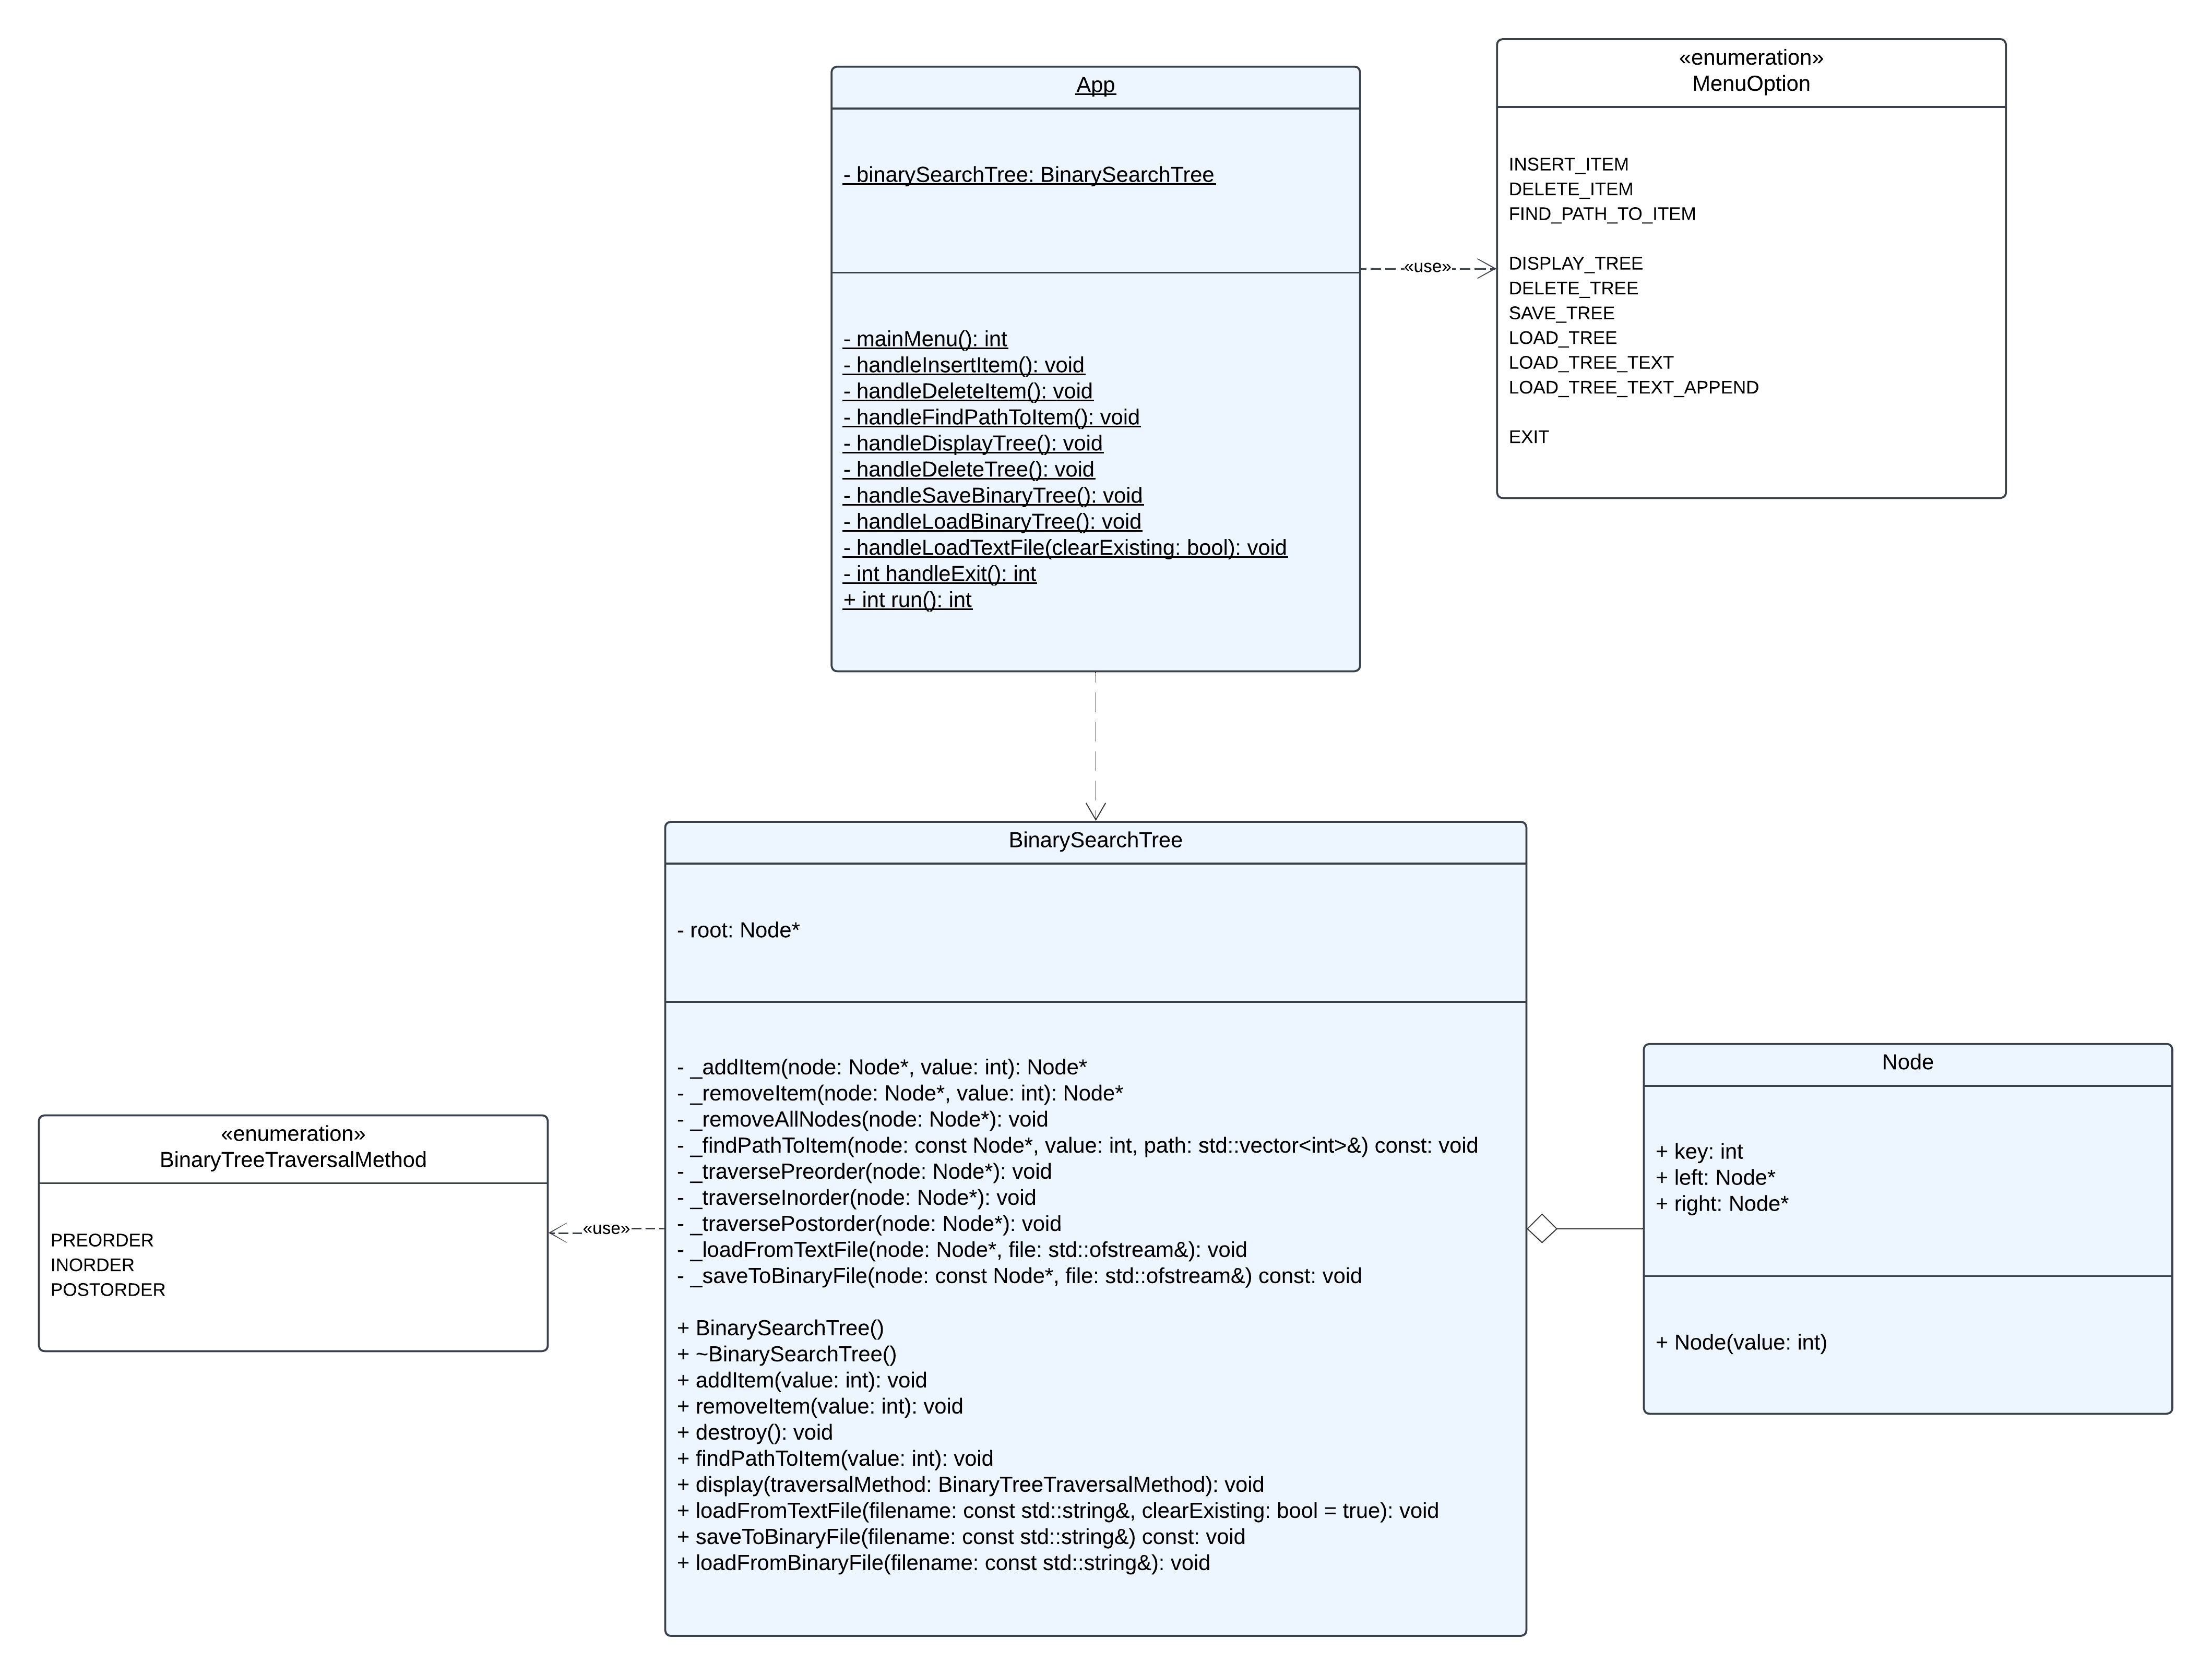
\includegraphics[width=0.8\textwidth]{uml_diagram.png}
% 	\caption{Diagram UML klas aplikacji - pokazuje zależności między klasami BinarySearchTree oraz App.}
% 	\label{fig:uml_diagram}
% \end{figure}

W projekcie zastosowano klasy \texttt{BinarySearchTree} oraz \texttt{App}. Klasa \texttt{BinarySearchTree} odpowiada za przechowywanie struktury drzewa oraz wykonanie operacji na drzewie (dodawanie, usuwanie, przeglądanie). Klasa \texttt{App} zapewnia interfejs użytkownika oraz umożliwia zarządzanie drzewem za pomocą menu.

\begin{itemize}
	\item \textbf{Klasa BinarySearchTree:} Przechowuje dane drzewa oraz implementuje operacje na nim, takie jak dodawanie elementów, usuwanie, przeglądanie w różnych metodach (preorder, inorder, postorder).
	\item \textbf{Klasa App:} Zapewnia menu, które umożliwia użytkownikowi interakcję z drzewem: dodawanie, usuwanie elementów oraz wyświetlanie struktury drzewa.
\end{itemize}

\subsection{Git i narzędzia CI/CD}

Projekt oparty jest na systemie kontroli wersji Git, z repozytorium umieszczonym na platformie GitHub. GitHub Actions jest wykorzystywane do automatyzacji procesu budowania i testowania projektu. Do weryfikacji wiadomości commitów stosowana jest konwencja \textit{Conventional Commits} i narzędzie \texttt{Commitlint}.

\subsection{Przykład użycia Git}

Poniżej przedstawiono przykładową procedurę pracy z projektem przy użyciu Git:

\begin{itemize}
	\item \textbf{Tworzenie nowego brancha:} Aby rozpocząć pracę nad nową funkcjonalnością, użytkownik tworzy nowy branch:
	      \begin{verbatim}
    git checkout -b feature-new-feature
    \end{verbatim}
	\item \textbf{Dodawanie zmian:} Po wprowadzeniu zmian, użytkownik dodaje je do systemu kontroli wersji:
	      \begin{verbatim}
    git add .
    \end{verbatim}
	\item \textbf{Commit zmian:} Następnie użytkownik wykonuje commit:
	      \begin{verbatim}
    git commit -m "feat: dodanie nowej funkcjonalności"
    \end{verbatim}
	\item \textbf{Wysyłanie zmian na GitHub:} Po wykonaniu kilku commitów, użytkownik wysyła zmiany do repozytorium:
	      \begin{verbatim}
    git push origin feature-new-feature
    \end{verbatim}
	\item \textbf{Scalanie zmian:} Po zakończeniu pracy nad funkcjonalnością, branch jest scalany do głównego brancha (np. \texttt{main}):
	      \begin{verbatim}
    git checkout main
    git pull origin main
    git merge feature-new-feature
    git push origin main
    \end{verbatim}
\end{itemize}

\subsection{Podsumowanie}

W projekcie wykorzystano szereg narzędzi i technologii, które pozwalają na skuteczną i efektywną pracę nad projektem. Dzięki zastosowaniu systemów takich jak Git oraz GitHub Actions, proces integracji i testowania jest zautomatyzowany, co umożliwia szybkie wykrywanie błędów oraz integrację nowych funkcjonalności. Dokumentacja generowana przez Doxygen oraz LaTeX zapewnia jasny i profesjonalny sposób dokumentowania projektu.

	\newpage
\section{Implementacja}		%4
%Opisać implementacje algorytmu/programu. Pokazać ciekawe fragmenty kodu
%Opisać powstałe wyniki (algorytmu/nrzędzia)



\newpage
\section{Wnioski}

W ramach przeprowadzonego projektu opracowano aplikację do zarządzania drzewem binarnym wyszukiwania (BST), której głównym celem było umożliwienie użytkownikowi wykonywania podstawowych operacji na drzewie, takich jak dodawanie, usuwanie elementów oraz wyświetlanie struktury drzewa. Po zakończeniu implementacji i przeprowadzeniu testów można sformułować następujące wnioski:

\subsection{Cel projektu i jego realizacja}

Celem projektu było zaprojektowanie i implementacja algorytmu, który umożliwia efektywne zarządzanie drzewem binarnym wyszukiwania oraz udostępnienie intuicyjnego interfejsu użytkownika w postaci menu tekstowego. Projekt został zrealizowany zgodnie z założeniami, a aplikacja umożliwia wykonanie podstawowych operacji na drzewie BST w sposób wydajny i bezbłędny. Wszystkie funkcje aplikacji, takie jak dodawanie, usuwanie oraz przeglądanie drzewa, działają zgodnie z oczekiwaniami.

\subsection{Możliwości rozwoju i optymalizacji}

Choć aplikacja spełnia swoje zadanie, istnieje kilka obszarów, które mogą zostać zoptymalizowane w przyszłości:

\begin{itemize}
	\item \textbf{Zbalansowanie drzewa:} Algorytm nie zapewnia automatycznego balansowania drzewa, co może prowadzić do pogorszenia wydajności operacji, szczególnie w przypadku wstawiania elementów w sposób uporządkowany. Zastosowanie algorytmów balansujących, takich jak drzewa AVL czy czerwono-czarne, mogłoby poprawić czas wykonywania operacji.
	\item \textbf{Interfejs użytkownika:} Aplikacja wykorzystuje jedynie interfejs tekstowy, co ogranicza jej funkcjonalność i wygodę użytkowania. Można rozważyć rozbudowę aplikacji o graficzny interfejs użytkownika (GUI), co poprawiłoby interaktywność programu.
	\item \textbf{Zarządzanie pamięcią:} W przyszłości warto rozważyć implementację inteligentnego zarządzania pamięcią, szczególnie w przypadku dużych drzew. Zastosowanie wskaźników smart pointers mogłoby pomóc w automatycznym zarządzaniu pamięcią, co zmniejszyłoby ryzyko wycieków pamięci.
\end{itemize}

\subsection{Podsumowanie}

Projekt umożliwił dogłębne zrozumienie i implementację algorytmu dla drzewa binarnego wyszukiwania, a także pozwolił na praktyczne zapoznanie się z zagadnieniami związanymi z operacjami na drzewach. Choć aplikacja działa zgodnie z wymaganiami, przyszła wersja projektu może zostać rozbudowana o dodatkowe funkcjonalności, optymalizacje i udoskonalenia, które umożliwią jej jeszcze lepszą skalowalność i wygodę użytkowania.

Przeprowadzona implementacja pokazuje, że algorytm wyszukiwania w drzewie binarnym jest jednym z fundamentalnych narzędzi w informatyce, które znajduje szerokie zastosowanie w różnych dziedzinach, takich jak bazy danych, kompilatory czy systemy plików. Projekt stanowi solidną podstawę do dalszych badań nad algorytmami strukturalnymi i ich zastosowaniem w praktyce.

\nocite{GitHubProject, GitHubProjectTemplate}



%%%%%%%%%%%%%%%%%%% koniec treść główna dokumentu %%%%%%%%%%%%%%%%%%%%%
\newpage
\addcontentsline{toc}{section}{Literatura}
\printbibliography

\newpage
\hypersetup{linkcolor=black}
\renewcommand{\cftparskip}{3pt}
\clearpage
\renewcommand{\cftloftitlefont}{\Large\bfseries\sffamily}
\listoffigures
\addcontentsline{toc}{section}{Spis rysunków}
\thispagestyle{fancy}

\newpage
\renewcommand{\cftlottitlefont}{\Large\bfseries\sffamily}
\def\listtablename{Spis tabel}
\addcontentsline{toc}{section}{Spis tabel}\listoftables
\thispagestyle{fancy}

\newpage
\renewcommand{\cftlottitlefont}{\Large\bfseries\sffamily}
\renewcommand\lstlistlistingname{Spis listingów}
\addcontentsline{toc}{section}{Spis listingów}\lstlistoflistings
\thispagestyle{fancy}



%lista rzeczy do zrobienia: wypisuje na koñcu dokumentu, patrz: pakiet todo.sty
\todos
%koniec listy rzeczy do zrobienia
\end{document}
